\chapter{Écosystèmes et structure trophique}\label{ch:b1:ecosystem-organization}

Une source d'une plaine calcaire déverse une eau si claire que l'on
peut compter depuis une barque chaque plante, chaque poisson et chaque
tortue. La lumière du soleil tombe sur les zostères à raison de
\qty{1.7}{} million de kilocalories par mètre carré et par an~; l'herbe
en stocke un pour cent~; les escargots et les tortues qui la broutent en
reçoivent un sixième~; les poissons qui mangent les escargots, un
dixième encore~; et l'unique héron du sommet vit sur un cent-millième de
ce qui est tombé sur l'eau. Tout \omterm{def:b1:ecosystem-organization:ecosystem}{écosystème} est bâti ainsi~: un flux
d'énergie qui entre une fois, passe des mangés aux mangeurs et repart
en chaleur, tandis que la matière qu'il déplace est recyclée. Ce
chapitre définit l'\omterm{def:b1:ecosystem-organization:ecosystem}{écosystème} et ses parties, la \omterm{def:b1:ecosystem-organization:niche}{niche} que chaque
espèce occupe, les \omterm{def:b1:ecosystem-organization:trophic}{niveaux trophiques} et les réseaux par lesquels
l'énergie circule, la productivité qui fixe la taille de l'ensemble, et
les façons de compter combien de sortes d'êtres y vivent.

\section{Écosystème et niche}

\begin{definition}[Écosystème, biotope, biocénose]\label{def:b1:ecosystem-organization:ecosystem}
\index{ecosysteme@écosystème}\index{biotope}\index{biocenose@biocénose}
Un \emph{écosystème} est l'ensemble des \omterm{def:b1:organism-environment:organism}{organismes} vivant en un lieu
défini, avec le milieu physique qu'ils occupent et avec lequel ils
échangent~: la \emph{biocénose} --- toutes les \omterm{def:b1:populations:population}{populations} de toutes les
espèces --- et le \emph{biotope} --- le sol, l'eau, l'air, la lumière et
le climat. Ses limites sont choisies selon la question~: un tronc en
décomposition, une mare, une forêt, un bassin océanique, la biosphère
entière. Un écosystème est un \omterm{def:b1:organism-environment:organism}{système ouvert}
(\cref{ch:b1:organism-environment})~: l'énergie le traverse, la matière
y circule en cycle et en franchit les bords, et sa structure est le
schéma de qui mange qui.
\end{definition}

\begin{definition}[Habitat et niche]\label{def:b1:ecosystem-organization:niche}
\index{niche ecologique@niche écologique}\index{habitat}
L'\emph{habitat} d'une espèce est le lieu où elle vit~; sa \emph{niche}
est la façon dont elle y vit~: l'ensemble complet des conditions
qu'elle tolère et des ressources qu'elle emploie --- température,
humidité, lumière, nourriture, heure d'activité, sites de nidification
--- chacune étant une dimension le long de laquelle l'espèce occupe un
intervalle. La \emph{niche fondamentale} est l'intervalle qu'elle
pourrait occuper seule~; la \emph{niche réalisée}, la part qu'elle
occupe effectivement en présence de concurrents et de prédateurs
(\cref{ch:b1:species-interactions}). Deux espèces de même niche ne
peuvent coexister longtemps en un même lieu~; les niches des espèces
qui coexistent diffèrent, et la \omterm{def:b1:ecosystem-organization:ecosystem}{biocénose} est un jeu de niches
emboîtées.
\end{definition}

\begin{omfigure}
\begin{tikzpicture}[font=\footnotesize, >=Stealth, line cap=round]
  \draw[->, thick] (0,0) -- (7.4,0) node[below left] {température};
  \draw[->, thick] (0,0) -- (0,5.2) node[below right, rotate=90, anchor=south east] {};
  \node[rotate=90, anchor=south] at (-0.4,2.6) {taille des proies};
  \draw[thick, omDef, fill=omDef!18] (3.6,2.6) ellipse (2.8 and 1.9);
  \node[omDef!80!black, anchor=south] at (2.5,3.7) {niche fondamentale};
  \draw[thick, omThm, fill=omThm!25] (2.9,2.3) ellipse (1.6 and 1.2);
  \node[omThm!80!black] at (2.9,2.3) {niche réalisée};
  \draw[thick, omProp, fill=omProp!25, opacity=0.8] (5.6,3.4) ellipse (1.5 and 1.1);
  \node[omProp!80!black, align=center] at (5.6,3.4) {niche du\\ concurrent};
  \node[anchor=north, align=center, gray] at (3.7,-0.5) {deux des nombreuses dimensions d'une niche~; le concurrent exclut l'espèce du recouvrement};
\end{tikzpicture}

{\small La \omterm{def:b1:ecosystem-organization:niche}{niche} comme volume dans un espace de conditions et de
ressources, dont deux dimensions sont dessinées. La \omterm{def:b1:ecosystem-organization:niche}{niche} fondamentale
est ce qu'une espèce pourrait occuper~; la \omterm{def:b1:ecosystem-organization:niche}{niche} réalisée est ce que ses
concurrents lui laissent.}
\end{omfigure}

\begin{example}[Cinq fauvettes dans une même épicéa]\label{ex:b1:ecosystem-organization:warblers}
Cinq espèces de petites fauvettes insectivores nichent dans les mêmes
pessières et mangent les mêmes insectes~; observées de près, chacune
cherche sa nourriture dans une partie différente de l'arbre --- la
cime, les aiguilles neuves de la périphérie, les branches moyennes, le
tronc et les branches basses, le sol en dessous --- et à des hauteurs et
des heures différentes. Leur \omterm{def:b1:ecosystem-organization:niche}{habitat} est unique~; leurs \omterm{def:b1:ecosystem-organization:niche}{niches} sont
cinq, et la forêt porte cinq espèces là où la nourriture seule n'en
laisserait prévoir qu'une.
\end{example}

\section{La structure trophique}

\begin{definition}[Producteurs, consommateurs, décomposeurs]\label{def:b1:ecosystem-organization:trophic}
\index{niveau trophique}\index{producteur}\index{consommateur}\index{decomposeur@décomposeur}
Les \omterm{def:b1:organism-environment:organism}{organismes} d'un \omterm{def:b1:ecosystem-organization:ecosystem}{écosystème} sont groupés selon ce qu'ils mangent en
\emph{niveaux trophiques}. Les \emph{producteurs} (autotrophes~:
plantes, algues, cyanobactéries, bactéries chimiosynthétiques)
fabriquent de la matière organique à partir de matière minérale~; ils
forment le premier niveau. Les \emph{consommateurs} la mangent~: les
\emph{consommateurs primaires} (herbivores) mangent les producteurs,
les \emph{consommateurs secondaires} (carnivores) mangent les
herbivores, les consommateurs \emph{tertiaires} mangent les carnivores~;
les omnivores mangent à plusieurs niveaux. Les \emph{décomposeurs}
(bactéries, champignons) et les \emph{détritivores} (vers de terre,
cloportes, bousiers) vivent de la matière morte et des déchets de tous
les niveaux, et rendent leurs minéraux au sol et à l'eau pour que les
producteurs les reprennent --- le maillon qui referme le cycle de la
matière.
\end{definition}

\begin{definition}[Chaîne alimentaire, réseau trophique]\label{def:b1:ecosystem-organization:foodweb}
\index{chaine alimentaire@chaîne alimentaire}\index{reseau trophique@réseau trophique}
Une \emph{chaîne alimentaire} est une suite d'\omterm{def:b1:organism-environment:organism}{organismes} mangeant
chacun le précédent~: herbe, criquet, grenouille, serpent, buse. Dans
une \omterm{def:b1:ecosystem-organization:ecosystem}{biocénose} réelle, chaque espèce en mange plusieurs et est mangée
par plusieurs, et les chaînes s'entrelacent en un \emph{réseau
trophique}, dont les flèches vont du mangé au mangeur --- dans le sens
de l'énergie. Les chaînes sont courtes~: rarement plus de quatre ou cinq
maillons, pour une raison que donne la section suivante.
\end{definition}

\begin{omfigure}
\begin{tikzpicture}[font=\footnotesize, >=Stealth, line cap=round,
  sp/.style={draw, thick, rounded corners=3pt, inner sep=3pt, align=center, fill=white}]
  \node[sp, fill=omExo!20] (grass) at (1.5,0) {zostères, algues};
  \node[sp, fill=omExo!20] (det) at (6.5,0) {détritus};
  \node[sp, fill=omProp!20] (snail) at (0,2.0) {escargots};
  \node[sp, fill=omProp!20] (insect) at (2.6,2.0) {larves d'insectes};
  \node[sp, fill=omProp!20] (turtle) at (5.0,2.0) {tortues};
  \node[sp, fill=omProp!20] (shrimp) at (7.6,2.0) {crevettes, vers};
  \node[sp, fill=omThm!20] (sunfish) at (1.3,4.0) {crapets};
  \node[sp, fill=omThm!20] (catfish) at (6.4,4.0) {poissons-chats};
  \node[sp, fill=omDef!25] (bass) at (2.8,5.8) {achigans};
  \node[sp, fill=omDef!25] (heron) at (6.0,5.8) {hérons};
  \node[sp, fill=gray!20] (dec) at (10.2,1.0) {bactéries, champignons\\ (décomposeurs)};
  \draw[->, thick] (grass) -- (snail); \draw[->, thick] (grass) -- (insect); \draw[->, thick] (grass) -- (turtle);
  \draw[->, thick] (det) -- (shrimp); \draw[->, thick] (det) -- (insect);
  \draw[->, thick] (snail) -- (sunfish); \draw[->, thick] (insect) -- (sunfish); \draw[->, thick] (insect) -- (catfish); \draw[->, thick] (shrimp) -- (catfish);
  \draw[->, thick] (sunfish) -- (bass); \draw[->, thick] (sunfish) -- (heron); \draw[->, thick] (catfish) -- (heron); \draw[->, thick] (catfish) -- (bass);
  \draw[->, thick] (turtle) -- (heron);
  \draw[->, thick, gray, dashed] (9.0,0.4) -- (dec); \node[gray, font=\scriptsize, anchor=north] at (9.0,0.3) {toute la matière morte};
  \node[anchor=east, omExo!70!black] at (-0.6,0) {producteurs};
  \node[anchor=east, omProp!80!black] at (-0.6,2.0) {consommateurs I};
  \node[anchor=east, omThm!80!black] at (-0.6,4.0) {consommateurs II};
  \node[anchor=east, omDef!80!black] at (-0.6,5.8) {consommateurs III};
\end{tikzpicture}

{\small Un \omterm{def:b1:ecosystem-organization:foodweb}{réseau trophique} simplifié d'une source claire. Les flèches
vont de la nourriture au mangeur, dans le sens du flux d'énergie~; la
plupart des espèces mangent à plus d'un niveau, et tout finit chez les
\omterm{def:b1:ecosystem-organization:trophic}{décomposeurs}.}
\end{omfigure}

\begin{omfigure}
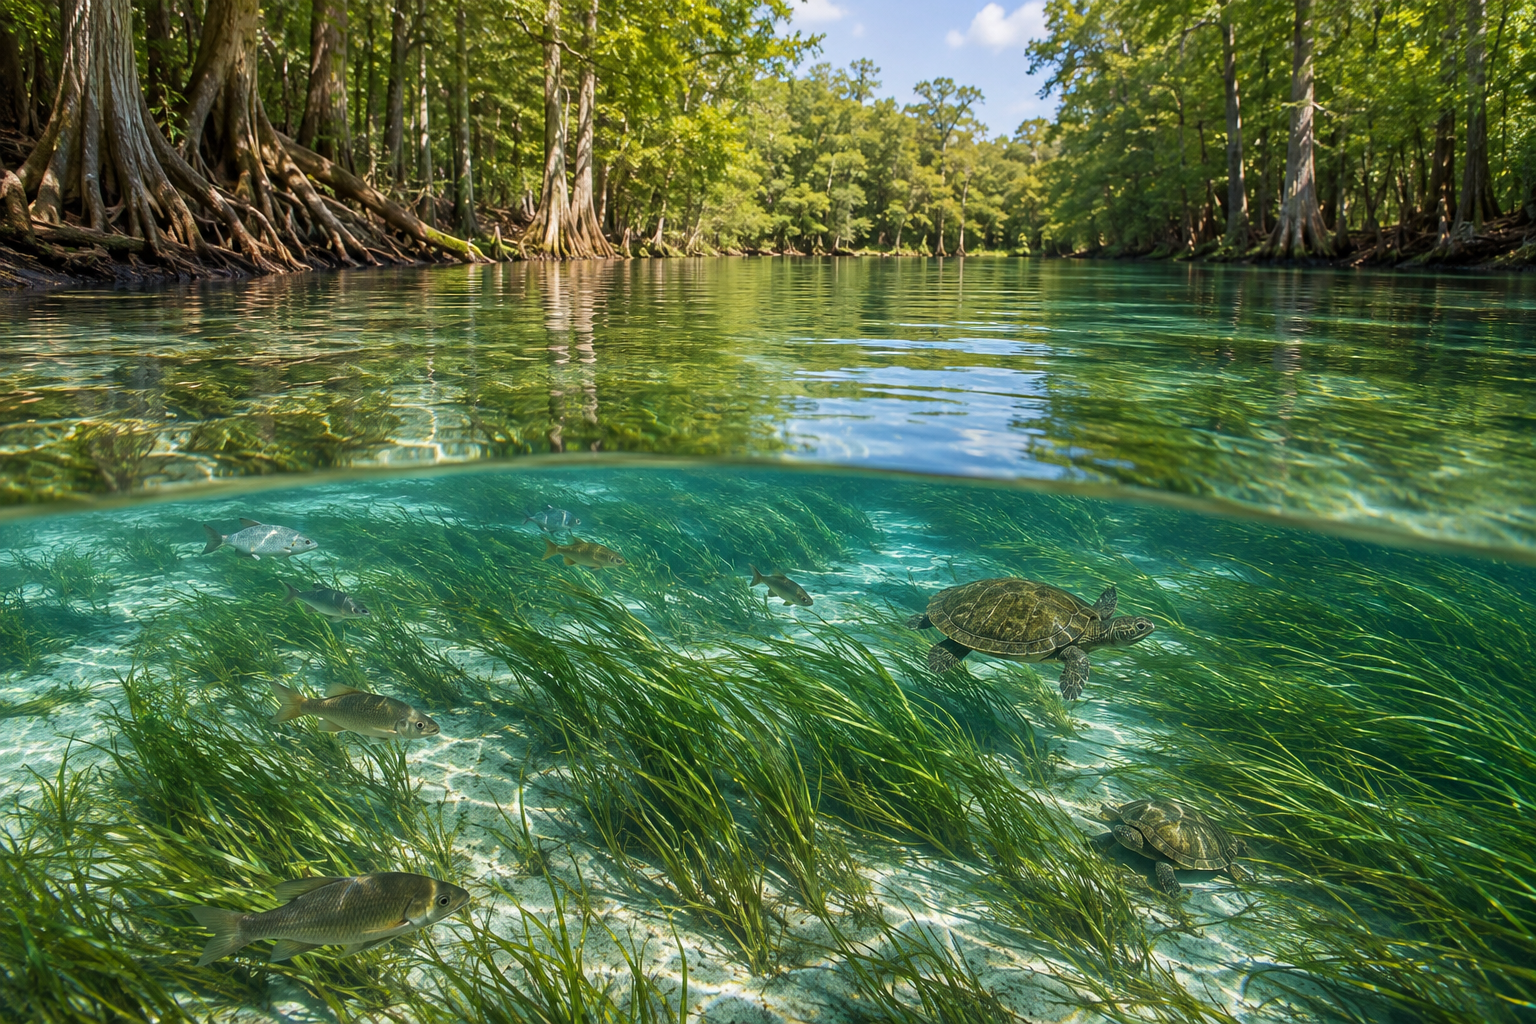
\includegraphics[width=0.6\linewidth]{images/book3/ai/b3-26-clear-spring.png}

{\small Une source calcaire~: une couche productrice de zostères et
d'algues en pleine lumière, et au-dessus les \omterm{def:b1:ecosystem-organization:trophic}{consommateurs} pour
lesquels fut dressé le premier bilan énergétique écologique.}
\end{omfigure}

\section{Le flux d'énergie}

\begin{definition}[Productivité]\label{def:b1:ecosystem-organization:productivity}
\index{productivite primaire@productivité primaire}\index{productivite primaire brute@productivité primaire brute}\index{productivite primaire nette@productivité primaire nette}
La \emph{productivité primaire brute} (PPB) d'un \omterm{def:b1:ecosystem-organization:ecosystem}{écosystème} est la
vitesse à laquelle ses \omterm{def:b1:ecosystem-organization:trophic}{producteurs} fixent de l'énergie par
photosynthèse, par unité d'aire et de temps
(\unit{kJ.m^{-2}.yr^{-1}}, ou en grammes de carbone ou de matière
sèche)~; la \emph{productivité primaire nette} (PPN) est ce qui reste
après la respiration des \omterm{def:b1:ecosystem-organization:trophic}{producteurs} eux-mêmes --- la matière organique
effectivement mise à la disposition du reste du système. La
\emph{productivité secondaire} est la vitesse à laquelle les
\omterm{def:b1:ecosystem-organization:trophic}{consommateurs} bâtissent leur propre biomasse à partir de ce qu'ils
mangent. La \emph{biomasse} est le stock présent à un instant~; la
productivité est un flux, la biomasse un stock, et le rapport des deux
est le temps de renouvellement.
\end{definition}

\begin{theorem}[La règle des dix pour cent]\label{thm:b1:ecosystem-organization:lindeman}
\index{efficacite trophique@efficacité trophique}
De l'énergie qui entre à un \omterm{def:b1:ecosystem-organization:trophic}{niveau trophique} sous forme de nourriture,
un dixième environ --- entre \qty{5}{} et \qty{20}{\%} --- atteint le
niveau suivant comme nourriture. Le reste n'est pas mangé, n'est pas
assimilé (il repart en fèces), ou est respiré par le niveau lui-même.
L'énergie disponible chute donc d'un facteur dix par niveau, ce qui
explique que les \omterm{def:b1:ecosystem-organization:foodweb}{chaînes alimentaires} dépassent rarement quatre ou cinq
maillons, et que la biomasse et les effectifs des prédateurs supérieurs
soient faibles.
\end{theorem}
\begin{proof}[Démonstration partielle]
L'énergie assimilée par un niveau est ce qu'il mange moins ce qu'il
excrète~; là-dessus, la respiration prend ce que le niveau dépense à
vivre (\cref{ch:b1:organism-environment}), et seul le reste --- sa
croissance et sa reproduction --- est disponible pour être mangé.
Chacune des trois fractions (mangé, assimilé, converti en biomasse) est
bien inférieure à un~: pour un herbivore de prairie, environ
\qty{20}{\%} de la croissance des plantes est mangée, \qty{50}{\%} de
cela est assimilé, et \qty{10}{\%} de cela est transformé en chair, ce
qui donne \qty{1}{\%}~; pour un carnivore, qui mange et assimile une
plus grande part de sa proie, environ \qty{10}{\%}. La règle est une
régularité observée, non une loi~; sa valeur est celle que donnent les
mesures.
\end{proof}
\begin{proof}[Faits expérimentaux]
Lindeman (1942) mesura, dans un petit lac, l'énergie fixée par le
plancton et l'énergie retenue puis respirée à chaque niveau au-dessus,
et trouva que chaque niveau en transmettait environ un dixième. Odum
(1957) dressa le bilan complet d'une source de Floride~: sur
\qty{1.7e6}{kcal} par mètre carré et par an de lumière solaire, les
\omterm{def:b1:ecosystem-organization:trophic}{producteurs} en fixèrent \num{20800} (brut), en respirèrent \num{12000}
et en laissèrent \num{8800} de net~; les herbivores en prélevèrent
\num{3400} et en transmirent \num{380} aux carnivores~; les carnivores
en transmirent \num{20} aux carnivores supérieurs. Les rendements
étaient de \qty{1.2}{\%}, \qty{16}{\%}, \qty{11}{\%} et \qty{5}{\%} ---
la règle des dix pour cent à un facteur deux près à chaque étape.
\end{proof}

\begin{omfigure}
\begin{tikzpicture}[font=\footnotesize, >=Stealth, line cap=round]
  % energy pyramid: widths proportional to log-ish scale of energy
  \fill[omExo!45] (-4.4,0) rectangle (4.4,0.9); \node at (0,0.45) {producteurs~: net \num{8800} kcal\,m$^{-2}$\,an$^{-1}$ (brut \num{20800})};
  \fill[omProp!45] (-2.9,1.1) rectangle (2.9,2.0); \node at (0,1.55) {herbivores~: \num{3400} prélevées, \num{1500} assimilées};
  \fill[omThm!45] (-1.5,2.2) rectangle (1.5,3.1); \node at (0,2.65) {carnivores~: \num{380}};
  \fill[omDef!45] (-0.5,3.3) rectangle (0.5,4.2); \node[anchor=south] at (0,4.25) {carnivores supérieurs~: \num{20}};
  \node[anchor=east, align=right] at (-4.6,0.45) {soleil~:\\ \num{1700000}};
  \node[anchor=east, align=right, gray] at (-3.1,1.55) {\qty{16}{\%}};
  \node[anchor=east, align=right, gray] at (-1.7,2.65) {\qty{11}{\%}};
  \node[anchor=east, align=right, gray] at (-0.7,3.75) {\qty{5}{\%}};
  \draw[->, thick, gray] (4.6,0.45) -- (5.4,0.45) node[right, align=left] {respiration et\\ décomposeurs~: chaleur};
  \draw[->, thick, gray] (3.1,1.55) -- (5.4,1.55); \draw[->, thick, gray] (1.7,2.65) -- (5.4,2.65); \draw[->, thick, gray] (0.7,3.75) -- (5.4,3.75);
\end{tikzpicture}

{\small Le bilan énergétique d'une source (kilocalories par mètre carré
et par an). Chaque niveau transmet au suivant un dixième environ de ce
qu'il reçoit~; le reste part en chaleur par la respiration, pour
l'essentiel celle des \omterm{def:b1:ecosystem-organization:trophic}{décomposeurs}.}
\end{omfigure}

\begin{proposition}[Les pyramides]\label{prop:b1:ecosystem-organization:pyramids}
\index{pyramide ecologique@pyramide écologique}
Empiler les \omterm{def:b1:ecosystem-organization:trophic}{niveaux trophiques} donne une \emph{pyramide}. Une pyramide
d'\emph{énergie} (le flux par niveau) est toujours droite~: chaque
niveau ne peut transmettre que moins qu'il n'a reçu. Une pyramide de
\emph{biomasse} (le stock présent) est d'ordinaire droite mais peut
être inversée~: en haute mer, le phytoplancton, mangé aussi vite qu'il
pousse, pèse à tout instant moins que le zooplancton qui en vit, parce
qu'il se renouvelle en quelques jours quand les animaux durent des
mois. Une pyramide des \emph{effectifs} peut prendre n'importe quelle
forme~: un seul chêne nourrit des milliers de chenilles. L'énergie est
la mesure honnête.
\end{proposition}

\begin{method}[Dresser un bilan énergétique]\label{met:b1:ecosystem-organization:budget}
\begin{enumerate}
  \item Mesurer la PPB~: par les échanges gazeux (oxygène dégagé ou
        $\mathrm{CO_2}$ absorbé par une parcelle ou un flacon à la
        lumière et à l'obscurité~: lumière moins obscurité donne le
        brut, la lumière seule donne le net), ou par la récolte
        (biomasse gagnée dans l'année plus ce qui a été mangé et perdu).
  \item Mesurer, pour chaque niveau de \omterm{def:b1:ecosystem-organization:trophic}{consommateurs}, l'ingestion (ce
        qu'il mange), l'assimilation (ingestion moins fèces), la
        respiration (sa consommation d'oxygène) et la production
        (croissance plus descendance $=$ assimilation moins
        respiration).
  \item \omterm{thm:b1:ecosystem-organization:lindeman}{Efficacité trophique} entre niveaux $=$ production du niveau
        supérieur $/$ production du niveau inférieur. Vérifier que la
        respiration, la production et la décomposition de chaque niveau
        totalisent son assimilation.
  \item Convertir en unités communes (\unit{kJ}, ou grammes de carbone
        à environ \qty{40}{kJ/g}) et tracer la pyramide~; la somme de
        toutes les respirations doit approcher la PPB sur une année
        dans un \omterm{def:b1:ecosystem-organization:ecosystem}{écosystème} stationnaire.
\end{enumerate}
\end{method}

\begin{example}[Pourquoi le sommet est mince]\label{ex:b1:ecosystem-organization:top}
Un kilomètre carré de savane produit quelque \qty{5000}{t} d'herbe par
an~; les brouteurs en font \qty{50}{t} d'antilopes et de buffles~; les
lions, \qty{2}{t} de lion --- un ou deux animaux. Pour nourrir un tigre,
une forêt doit être assez vaste pour que son dixième de dixième de
dixième de la lumière solaire fasse un cerf entier par semaine~: cent
kilomètres carrés par tigre, ce qui explique que les grands carnivores
soient rares, parcourent de longues distances, et disparaissent les
premiers quand un \omterm{def:b1:ecosystem-organization:niche}{habitat} se réduit.
\end{example}

\begin{proposition}[La productivité des biomes]\label{prop:b1:ecosystem-organization:biomes}
\index{biome}
La \omterm{def:b1:ecosystem-organization:productivity}{productivité primaire nette} par unité d'aire est fixée par la
lumière, la température, l'eau et les éléments nutritifs~: forêt
tropicale humide \qtyrange{2000}{3500}{} g de matière sèche par mètre
carré et par an~; forêt tempérée et terres cultivées
\qtyrange{600}{1500}{}~; prairie \qtyrange{200}{1500}{}~; toundra et
désert sous \qty{200}{}~; haute mer environ \qty{125}{} (lumière
abondante, éléments nutritifs rares), côtes d'upwelling et récifs
\qtyrange{500}{2500}{}. L'océan, les deux tiers de la planète, fournit
environ la moitié de la production mondiale~; les forêts, un dixième des
terres, en fournissent le tiers pour le domaine continental. Là où
l'eau et les éléments nutritifs abondent, la productivité suit la
lumière et la chaleur~; là où ils manquent, elle les suit, eux.
\end{proposition}

\begin{omfigure}
\begin{tikzpicture}
\begin{axis}[
  xbar, bar width=8pt,
  width=0.84\linewidth, height=6.6cm,
  axis x line=bottom, axis y line=left,
  xmin=0, xmax=2600, xlabel={productivité primaire nette (\unit{g.m^{-2}.yr^{-1}}, matière sèche)},
  xlabel style={font=\small, at={(axis description cs:0.5,-0.12)}, anchor=north},
  symbolic y coords={desert, ocean, toundra, prairie, cultures, foret temperee, estuaires, foret tropicale},
  yticklabels={désert, haute mer, toundra, prairie tempérée, terres cultivées, forêt tempérée, estuaires et récifs, forêt tropicale humide},
  ytick=data, tick label style={font=\small},
  enlarge y limits=0.08, xtick={0,500,1000,1500,2000,2500},
  nodes near coords, nodes near coords style={font=\scriptsize, anchor=west},
]
\addplot[fill=omExo!45, draw=omExo] coordinates {(90,desert) (125,ocean) (140,toundra) (600,prairie) (650,cultures) (1200,foret temperee) (1800,estuaires) (2200,foret tropicale)};
\end{axis}
\end{tikzpicture}

{\small \omterm{def:b1:ecosystem-organization:productivity}{Productivité primaire nette} moyenne des principaux biomes. Un
écart de un à vingt, fixé par l'eau, la chaleur, la lumière et les
éléments nutritifs.}
\end{omfigure}

\begin{omfigure}
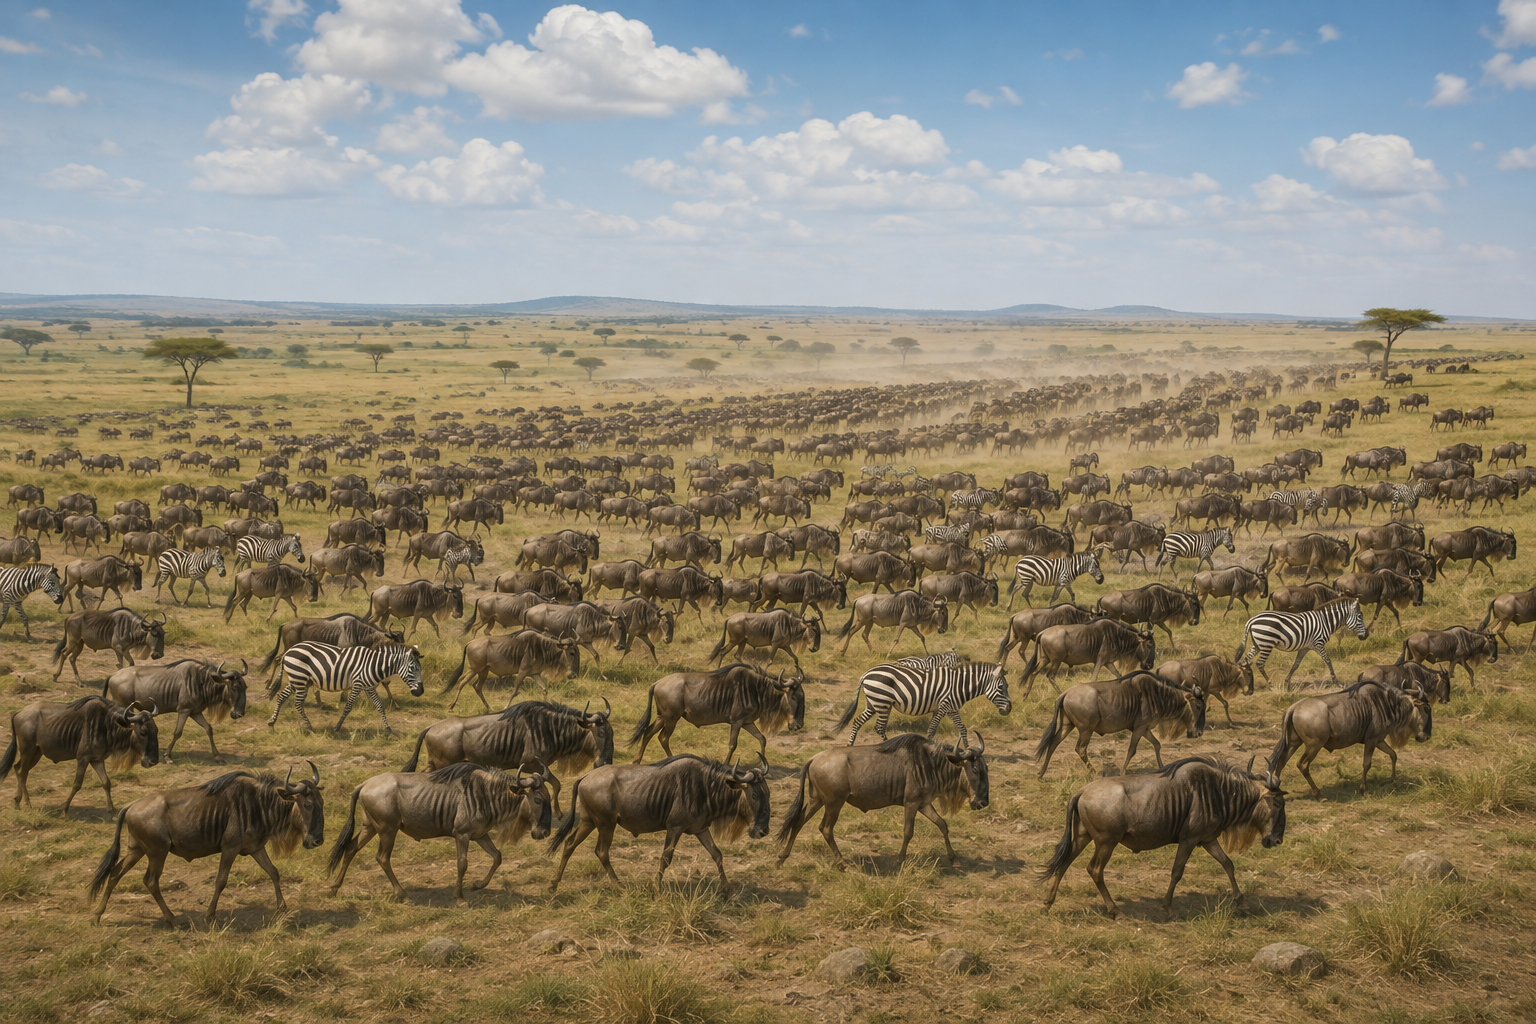
\includegraphics[width=0.6\linewidth]{images/book3/ai/b3-26-wildebeest-migration.png}

{\small Des brouteurs dans une savane~: un niveau de \omterm{def:b1:ecosystem-organization:trophic}{consommateurs}
primaires fort d'un million d'animaux, qui suit les pluies fixant la
productivité de l'herbe et porte un dixième de son énergie aux
prédateurs qui les suivent.}
\end{omfigure}

\section{Compter la diversité}

\begin{definition}[Richesse spécifique, indice de diversité]\label{def:b1:ecosystem-organization:diversity}
\index{richesse specifique@richesse spécifique}\index{indice de Shannon}
La \emph{richesse spécifique} $S$ d'une \omterm{def:b1:ecosystem-organization:ecosystem}{biocénose} est le nombre
d'espèces qu'elle contient. La richesse seule ignore l'abondance~: un
bois de cent chênes et d'un individu de chacun de neuf autres arbres
est moins divers qu'un bois de dix individus de chacun.
L'\emph{indice de Shannon}
\[
H = -\sum_{i=1}^{S} p_i \ln p_i ,
\]
où $p_i$ est la fraction des individus appartenant à l'espèce $i$,
croît avec la richesse et avec l'\emph{équitabilité}~; il vaut $\ln S$
quand toutes les espèces sont également abondantes et est proche de
zéro quand une seule domine. L'\emph{équitabilité} vaut $H/\ln S$. La
diversité croît généralement des pôles vers les tropiques, avec l'aire,
avec le temps écoulé depuis la dernière perturbation, et avec la
productivité du site jusqu'à un certain point.
\end{definition}

\begin{method}[Échantillonner une biocénose]\label{met:b1:ecosystem-organization:sampling}
\begin{enumerate}
  \item Échantillonner par une méthode adaptée aux \omterm{def:b1:organism-environment:organism}{organismes}
        (quadrats, filets, pièges, transects) et noter le nombre
        d'individus de chaque espèce.
  \item Porter le nombre d'espèces trouvées en fonction du nombre
        d'échantillons (ou d'individus)~: la courbe monte vite, puis
        s'aplatit~; là où elle s'aplatit, la richesse est presque
        complète. Ne comparer des \omterm{def:b1:ecosystem-organization:ecosystem}{biocénoses} qu'à effort
        d'échantillonnage égal.
  \item Calculer $H$ et l'équitabilité~; comparer avec le diagramme
        rang--abondance (espèces classées par abondance, en échelle
        logarithmique), dont la pente montre la dominance.
  \item Interpréter~: une faible équitabilité signale une espèce
        dominante ou un stress~; une baisse de $H$ au fil du temps
        signale un changement du \omterm{def:b1:ecosystem-organization:ecosystem}{biotope}.
\end{enumerate}
\end{method}

\begin{example}[Deux bois]\label{ex:b1:ecosystem-organization:twowoods}
Bois A~: 100 chênes et un individu de chacun de neuf autres arbres~;
$H = -(0.917\ln
0.917 + 9\times 0.0092\ln 0.0092) = 0.08 + 0.39 = 0.47$, équitabilité
$0.47/2.30 = 0.20$. Bois B~: dix individus de chacune des mêmes dix
espèces~; $H =
\ln 10 = 2.30$, équitabilité 1. Même richesse, cinq fois la diversité.
\end{example}

\section{Exercices}

\begin{exercise}[$\star$]\label{exo:b1:ecosystem-organization:1}
Définir \omterm{def:b1:ecosystem-organization:ecosystem}{écosystème}, \omterm{def:b1:ecosystem-organization:ecosystem}{biocénose} et \omterm{def:b1:ecosystem-organization:ecosystem}{biotope}, sur l'exemple d'une mare.
\end{exercise}

\begin{exercise}[$\star$]\label{exo:b1:ecosystem-organization:2}
Distinguer \omterm{def:b1:ecosystem-organization:niche}{habitat} et \omterm{def:b1:ecosystem-organization:niche}{niche}, puis \omterm{def:b1:ecosystem-organization:niche}{niche} fondamentale et \omterm{def:b1:ecosystem-organization:niche}{niche} réalisée.
\end{exercise}

\begin{exercise}[$\star$]\label{exo:b1:ecosystem-organization:3}
À partir de la pyramide énergétique de la source, calculer le rendement
de la lumière solaire à la production brute, et la fraction de la
production nette que les herbivores ont prélevée.
\end{exercise}

\begin{exercise}[$\star$]\label{exo:b1:ecosystem-organization:4}
Nommer les quatre groupes trophiques et dire lequel referme le cycle de
la matière.
\end{exercise}

\begin{exercise}[$\star\star$]\label{exo:b1:ecosystem-organization:5}
La PPN d'une prairie vaut \qty{800}{g.m^{-2}.yr^{-1}} (\qty{17}{kJ/g}).
Des lapins en mangent \qty{15}{\%}, assimilent \qty{50}{\%} de ce
qu'ils mangent, et transforment \qty{5}{\%} de ce qu'ils assimilent en
lapin. Calculer la production de lapin par hectare et l'\omterm{thm:b1:ecosystem-organization:lindeman}{efficacité
trophique} de la PPN au lapin.
\end{exercise}

\begin{exercise}[$\star\star$]\label{exo:b1:ecosystem-organization:6}
Expliquer pourquoi une pyramide de biomasse peut être inversée en mer
alors qu'une pyramide d'énergie ne l'est jamais.
\end{exercise}

\begin{exercise}[$\star\star$]\label{exo:b1:ecosystem-organization:7}
Calculer l'\omterm{def:b1:ecosystem-organization:diversity}{indice de Shannon} et l'équitabilité d'un échantillon de
50 A, 30 B, 15 C et 5 D. Comparer avec quatre espèces à 25 chacune.
\end{exercise}

\begin{exercise}[$\star\star$]\label{exo:b1:ecosystem-organization:8}
Dans une expérience de flacons clair et sombre, l'oxygène du flacon
clair monte de \qty{3}{mg/L} en un jour et celui du flacon sombre
baisse de \qty{1}{mg/L}. Calculer la productivité brute et nette de
l'eau en milligrammes d'oxygène par litre et par jour, puis en grammes
de carbone (\qty{1}{g} de $\mathrm{O_2}$ $\approx$ \qty{0.375}{g} de C).
\end{exercise}

\begin{exercise}[$\star\star$]\label{exo:b1:ecosystem-organization:9}
Pourquoi n'existe-t-il pas de \omterm{def:b1:ecosystem-organization:foodweb}{chaînes alimentaires} à dix maillons, et
pourquoi les îles et les déserts ont-ils des chaînes plus courtes que
les forêts~?
\end{exercise}

\begin{exercise}[$\star\star\star$]\label{exo:b1:ecosystem-organization:10}
Un humain peut manger du grain directement ou le donner à des bovins.
Avec une \omterm{thm:b1:ecosystem-organization:lindeman}{efficacité trophique} de \qty{10}{\%} pour les bovins,
calculer la surface nécessaire pour nourrir une personne au bœuf plutôt
qu'au grain, si le champ rend \qty{6}{t} de grain par hectare et qu'une
personne a besoin de \qty{1}{t} par an. Que dit ce calcul du \omterm{def:b1:ecosystem-organization:trophic}{niveau
trophique} humain et de la \omterm{thm:b1:populations:logistic}{capacité de charge} de la planète~?
\end{exercise}

\begin{exercise}[$\star\star\star$]\label{exo:b1:ecosystem-organization:11}
La haute mer a une faible PPN par mètre carré mais fournit la moitié de
la production mondiale. Concilier les deux, et expliquer pourquoi les
pêcheries de l'océan sont concentrées sur quelques pour cent de son
étendue.
\end{exercise}

\begin{exercise}[$\star\star\star$]\label{exo:b1:ecosystem-organization:12}
«~Un \omterm{def:b1:ecosystem-organization:ecosystem}{écosystème} est une machine à convertir la lumière du soleil en
chaleur, la vie n'en étant que le sous-produit.~» Discuter en un
paragraphe~: flux d'énergie contre cycle de la matière, ce que font les
\omterm{def:b1:ecosystem-organization:trophic}{décomposeurs}, et ce que la phrase laisse de côté.
\end{exercise}

\section{Problème~: le bilan d'une source}

\begin{problem}[{Problème du week-end --- la source d'Odum dressée
niveau par niveau~: du soleil à l'herbe, de l'herbe à l'escargot, de
l'escargot au poisson, du poisson au héron, avec les respirations et
les décomposeurs, jusqu'aux efficacités trophiques de chaque niveau}]
\label{pb:b1:ecosystem-organization:1}
Une source reçoit \qty{1.7e6}{kcal} de lumière solaire par mètre carré
et par an. Ses \omterm{def:b1:ecosystem-organization:trophic}{producteurs} en fixent \qty{20800}{kcal} (brut) et en
respirent \qty{12000}{}. Les herbivores mangent \qty{3400}{kcal} de
matière végétale, dont ils assimilent \qty{1500}{}, respirent
\qty{1100}{} et transforment le reste en croissance et en descendance.
Les carnivores mangent \qty{380}{kcal}, en respirent \qty{300}{} et
produisent le reste~; les carnivores supérieurs mangent \qty{20}{kcal},
en respirent \qty{14}{} et produisent \qty{6}{}. Tout ce qui n'est ni
mangé ni respiré va aux \omterm{def:b1:ecosystem-organization:trophic}{décomposeurs}, qui le respirent. Prendre
\qty{1}{kcal} $= \qty{4.18}{kJ}$ et \qty{10}{kcal} par gramme de
biomasse sèche.

\medskip
\noindent\textbf{Partie I --- Les \omterm{def:b1:ecosystem-organization:trophic}{producteurs}.}
\begin{enumerate}
  \item Calculer la \omterm{def:b1:ecosystem-organization:productivity}{productivité primaire nette}.
  \item Calculer le rendement de la photosynthèse~: production brute
        sur lumière solaire. Comparer avec les \qty{34}{\%} du
        \cref{ch:b1:photosynthesis} et citer trois pertes qui les
        séparent.
  \item Quelle fraction de la production brute les \omterm{def:b1:ecosystem-organization:trophic}{producteurs}
        respirent-ils~?
  \item Quelle part de la production nette est mangée par les
        herbivores, et quelle part va directement aux \omterm{def:b1:ecosystem-organization:trophic}{décomposeurs}~?
  \item Exprimer la PPN en grammes de matière sèche par mètre carré et
        par an et situer la source parmi les biomes du chapitre.
  \item Quelle part de la lumière solaire, par mètre carré et par an,
        quitte la source en chaleur sans jamais avoir traversé un être
        vivant~?
\end{enumerate}

\medskip
\noindent\textbf{Partie II --- Les \omterm{def:b1:ecosystem-organization:trophic}{consommateurs}.}
\begin{enumerate}[resume]
  \item Calculer la production des herbivores et leur efficacité
        d'assimilation (assimilé/mangé).
  \item Calculer l'efficacité de production des herbivores
        (production/assimilé).
  \item Calculer l'\omterm{thm:b1:ecosystem-organization:lindeman}{efficacité trophique} des \omterm{def:b1:ecosystem-organization:trophic}{producteurs} aux
        herbivores~: production des herbivores sur production primaire
        nette.
  \item Calculer la production des carnivores et l'\omterm{thm:b1:ecosystem-organization:lindeman}{efficacité
        trophique} des herbivores aux carnivores.
  \item Calculer l'\omterm{thm:b1:ecosystem-organization:lindeman}{efficacité trophique} des carnivores aux carnivores
        supérieurs.
  \item Combien d'énergie par mètre carré et par an atteint les \omterm{def:b1:body-plans-tissues:tissue}{tissus}
        mêmes du carnivore supérieur~? Quelle fraction de la lumière
        solaire cela représente-t-il~?
  \item Pourquoi l'efficacité d'assimilation croît-elle des herbivores
        aux carnivores~?
\end{enumerate}

\medskip
\noindent\textbf{Partie III --- Les \omterm{def:b1:ecosystem-organization:trophic}{décomposeurs} et le bilan.}
\begin{enumerate}[resume]
  \item Énumérer tous les flux vers les \omterm{def:b1:ecosystem-organization:trophic}{décomposeurs} (production nette
        non mangée, fèces des herbivores et production d'herbivores non
        mangée, et ainsi de suite) et en faire la somme.
  \item Calculer la respiration totale de l'\omterm{def:b1:ecosystem-organization:ecosystem}{écosystème}~: \omterm{def:b1:ecosystem-organization:trophic}{producteurs},
        herbivores, carnivores, carnivores supérieurs et \omterm{def:b1:ecosystem-organization:trophic}{décomposeurs}.
  \item La comparer à la production brute. Que signifie cette
        comparaison pour la biomasse de la source sur une année~?
  \item Quelle fraction de la production brute les \omterm{def:b1:ecosystem-organization:trophic}{décomposeurs}
        respirent-ils~?
  \item Tracer la pyramide d'énergie avec la production des quatre
        niveaux et y porter les efficacités.
\end{enumerate}

\medskip
\noindent\textbf{Partie IV --- Stocks, renouvellement et changement.}
La biomasse présente est de \qty{800}{g/m^2} de \omterm{def:b1:ecosystem-organization:trophic}{producteurs},
\qty{40}{g/m^2} d'herbivores, \qty{10}{g/m^2} de carnivores et
\qty{1.5}{g/m^2} de carnivores supérieurs.
\begin{enumerate}[resume]
  \item Convertir chaque biomasse en kilocalories et tracer la
        pyramide de biomasse. Est-elle droite~?
  \item Calculer le temps de renouvellement (biomasse/production) de
        chaque niveau. Lequel se renouvelle le plus vite, et pourquoi~?
  \item Un héron de \qty{2}{kg} vit de la production des carnivores
        supérieurs de la source. De combien de mètres carrés a-t-il
        besoin~?
  \item La source est enrichie d'engrais et sa production brute double,
        mais les herbivores ne peuvent manger plus vite. Qu'advient-il
        de la production supplémentaire, de la respiration des
        \omterm{def:b1:ecosystem-organization:trophic}{décomposeurs} et de l'oxygène de l'eau la nuit~?
  \item On introduit un nouveau poisson qui mange les œufs des
        herbivores et divise leur production par deux. Prévoir la
        production des carnivores et le nombre de hérons, ainsi que le
        sort des zostères.
  \item Expliquer pourquoi retirer les carnivores supérieurs
        changerait les zostères bien davantage que retirer l'équivalent
        énergétique en herbivores.
  \item Énoncer le résultat~: les \omterm{thm:b1:ecosystem-organization:lindeman}{efficacités trophiques} à chacun des
        trois transferts, le rendement de la lumière solaire à la
        production brute, et la fraction de l'énergie du soleil qui
        atteint les carnivores supérieurs.
\end{enumerate}
\end{problem}
